\chapter{Metodologia}
% ---

\section{Conteúdos específicos do modelo de trabalho acadêmico}

Em todos os conteúdos, sejam quadros, tabelas, figuras ou códigos, você pode usar o comando \verb|\fonte{CITE A FONTE AQUI}| e o texto com a fonte irá aparecer abaixo do conteúdo. Todos os exemplos abaixo estão usando.

\subsection{Quadros}

Este modelo vem com o ambiente \texttt{quadro} e impressão de Lista de quadros configurados por padrão. Verifique um exemplo de utilização:

\begin{quadro}[htb]
\caption{\label{quadro_exemplo}Exemplo de quadro}
\begin{tabular}{|c|c|c|p{3cm}|}
	\hline
	\textbf{Pessoa} & \textbf{Idade} & \textbf{Peso} & \textbf{Altura} \\ \hline
	Marcos & 26    & 68   & 178    \\ \hline
	Ivone  & 22    & 57   & 162    \\ \hline
	...    & ...   & ...  & ...    \\ \hline
	Sueli  & 40    & 65   & 153    \\ \hline
\end{tabular}
\fonte{Autor?}
\end{quadro}

Este parágrafo apresenta como referenciar o quadro no texto, requisito obrigatório da ABNT.  Primeira opção, utilizando \texttt{autoref}: Ver o \autoref{quadro_exemplo}.  Segunda opção, utilizando  \texttt{ref}: Ver o Quadro \ref{quadro_exemplo}.

Para entender a diferença entre tabela e quadro, o conteúdo em \url{https://www.significados.com.br/tabelas-quadros-e-figuras/} pode ajudar. As listas de quadros e de tabelas são geradas automaticamente e só aparecem se o trabalho tiver pelo menos um quadro ou uma tabela.

\subsection{Tabelas}

Utilize o ambiente \texttt{table} para inserir tabelas no seu trabalho. O exemplo a seguir mostra como adicionar uma tabela, definir uma legenda e referenciá-la no texto conforme as normas da ABNT. Para referenciar, utilize \texttt{autoref} (por exemplo, veja a \autoref{tabela_exemplo1}) ou \texttt{ref} (por exemplo, veja a Tabela \ref{tabela_exemplo1}).

\begin{table}[h!tb]
\centering
\caption{Exemplo de tabela}
\label{tabela_exemplo1}
\begin{tabular}{ccc}
\hline
\textbf{Coluna 1} & \textbf{Coluna 2} & \textbf{Coluna 3} \\ \hline
Dado 1 & Dado 2 & Dado 3 \\ \hline
Dado 4 & Dado 5 & Dado 6 \\ \hline
Dado 7 & Dado 8 & Dado 9 \\ \hline
\end{tabular}
\fonte{Acho que também não é do Autor.}
\end{table}

\subsection{Figuras}

Utilize o ambiente \texttt{figure} para inserir figuras no seu trabalho. O exemplo a seguir mostra como adicionar uma figura, definir uma legenda e referenciá-la no texto conforme as normas da ABNT. Para referenciar, utilize \texttt{autoref} (por exemplo, veja a \autoref{figura_exemplo1}) ou \texttt{ref} (por exemplo, veja a Figura \ref{figura_exemplo2}).

\begin{figure}[h!tb]
\centering
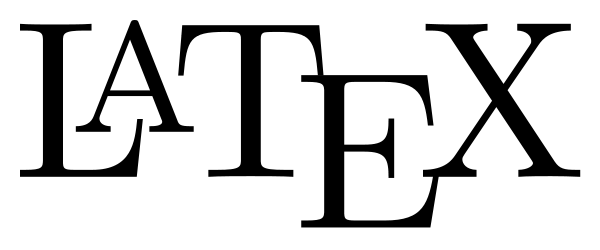
\includegraphics[width=0.5\textwidth]{figuras/LaTeX_logo.png}
\caption{Logo do \LaTeX (e png transparente).}
\label{figura_exemplo1}
\fonte{Algum lugar da internet.}
\end{figure}

\begin{figure}[h!tb]
\centering

\includegraphics[width=0.5\textwidth]{figuras/Luva_latex.png}
\caption{Não é o logo do \LaTeX (e não é um png transparente).}
\label{figura_exemplo2}
\fonte{Algum outro lugar da internet.}
\end{figure}

Você também pode colocar as figuras lado a lado, com um caption para cada uma, utilizando o ambiente \texttt{subcaption}. Não utilize o pacote \texttt{subfig}, pois já está defasado e levanta erros na compilação.

\begin{figure}[htbp]
    \centering
    \begin{subfigure}[b]{0.45\textwidth}
        \centering
        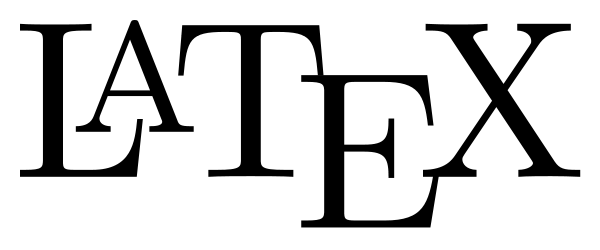
\includegraphics[width=\textwidth]{figuras/LaTeX_logo.png}
        \caption{Logo do \LaTeX.}
        {\label{figura_lado_a_lado1}}
        \fonte{Algum lugar da internet.}
    \end{subfigure}
    \hfill
    \begin{subfigure}[b]{0.45\textwidth}
        \centering
        
\includegraphics[width=\textwidth]{figuras/Luva_latex.png}
        \caption{Luva de latex.}
        \label{figura_lado_a_lado2}
        \fonte{Algum outro lugar da internet.}
    \end{subfigure}
    \caption{Exemplo de figuras lado a lado.}
    \label{figuras_lado_a_lado}
    \fonte{Não é do Autor (2026)}
\end{figure}

Agora, você pode referenciar as figuras lado a lado com \texttt{autoref} (por exemplo, veja a \autoref{figuras_lado_a_lado} e a e \autoref{figura_lado_a_lado1}), ou com \texttt{ref} (por exemplo, veja as Figuras \ref{figura_lado_a_lado1} e \ref{figura_lado_a_lado2}).

Lembrando que os códigos para as figuras você pode conferir direto nos arquivos .tex. No pdf final, só elas vão aparecer, sem o código fonte. A lista de ilustrações só aparece se o trabalho tiver pelo menos uma figura.

\subsection{Algoritmos}

Para citar trechos de códigos, você pode usar o ambiente \texttt{algorithm} em conjunto com com o pacote \texttt{minted}. Além de colorir o código de acordo com cada linguagem, permitem referenciar como Algoritmos ao invés de figuras ou tabelas, criando uma nova lista no sumário. Veja exemplos em Python e C:

\begin{algorithm}[H]
\caption{Busca Binária em Python}
\label{exemplo_codigo_python}
\begin{minted}{python}
def busca_binaria(arr, alvo):
    inicio, fim = 0, len(arr) - 1
    while inicio <= fim:
        meio = (inicio + fim) // 2
        if arr[meio] == alvo:
            return meio
        elif arr[meio] < alvo:
            inicio = meio + 1
        else:
            fim = meio - 1
    return -1
\end{minted}
\fonte{Autor (2026)}
\end{algorithm}

\begin{algorithm}[H]
\caption{Hello World em C}
\label{exemplo_codigo_c}
\begin{minted}{c}
#include <stdio.h>

int main() {
    printf("Hello, World!\n");
    return 0;
}
\end{minted}
\fonte{Autor (2026)}
\end{algorithm}

Referencie seus códigos com o pacote \texttt{autoref}, como \autoref{exemplo_codigo_python} ou \autoref{exemplo_codigo_c}. Você também pode referenciar o código no texto usando \texttt{ref} (por exemplo, veja o Algoritmo \ref{exemplo_codigo_python} e o Algoritmo \ref{exemplo_codigo_c}). A lista de algoritmos só aparece se o trabalho tiver pelo menos um algoritmo.

\section{Declaração sobre uso de Inteligência Artificial}

Se você utilizou ferramentas de IA como apoio da sua pesquisa, você precisa declarar aqui detalhadamente onde e como cada modelo foi utilizado. Liste todas as ferramentas e onde foram utilizadas, citando também versão, modelo, etc.

Adaptando o modelo sugerido no blog da Dra. Nathalia Cavichiolli~\footnote{Link: https://www.doutoranathalia.com.br/blog/como-declarar-uso-de-ia-no-trabalho-academico/}, fica a sugestão abaixo para utilização:

“Para a produção deste trabalho, foi utilizado [nome da ferramenta] ([empresa], [versão/data de acesso]) para [finalidade específica: revisão gramatical / geração de estrutura inicial / síntese de literatura / tradução de trechos / outro]. O uso ocorreu nas seguintes etapas: [especificar]. Todo conteúdo gerado pela ferramenta foi revisado criticamente pelo/a/os/as autor/a/es/as, que assume/m integral responsabilidade pelo trabalho final.”

Sobre este modelo, dois modelos foram usados para resolver um bug que surgiu após modificar as regras para avaliadores, quebrando a contra-capa e folha de rosto. Assim, esta seção deve ter o texto a seguir: 

Para a produção deste trabalho, foram utilizados os modelos Sonnet 5.5 (Anthropic) e Opus 5.5 (Anthropic) para correção de bugs na geração da contra-capa e folha de rosto. Todo conteúdo gerado pela ferramenta foi revisado criticamente pelo autor, que assume integral responsabilidade pelo trabalho final.